\documentclass[11pt,a4paper,twoside]{article}
\usepackage[margin=1in, headheight=14pt]{geometry}
\usepackage{amsfonts,amsmath,amssymb,suetterl}
\usepackage{lmodern}
\usepackage[T1]{fontenc}
\usepackage{fancyhdr}
\usepackage{float}
\usepackage[utf8]{inputenc}
\usepackage{fontawesome}
\usepackage{enumerate}

\usepackage{tikz}
\usetikzlibrary{patterns, arrows.meta}

\DeclareUnicodeCharacter{2212}{-}

\usepackage{mathrsfs}
\usepackage[nodisplayskipstretch]{setspace}

\setstretch{1.5}
\renewcommand{\footrulewidth}{0pt}

\parindent 0ex
\setlength{\parskip}{1em}

\fancyfoot{}
\raggedbottom

% title page
\long\def\mytitle{
	\begin{titlepage}
		\begin{center}
			\Huge Queen Mary\\
			\LARGE University of London
		\end{center}

		\vspace*{\stretch{1}}

		\begin{singlespace}
			{\centering
					{\huge\bfseries MTH5123 Differential Equations\\}
					\vspace{0.5cm}

					{\Large Lecture Notes\\}
					\vspace{0.5cm}

					{\Large Week 1}

					\vfill
					\LARGE Weini Huang
					\vspace{0.5cm}
					
					\LARGE School of Mathematical Sciences\\
					\LARGE Queen Mary University of London\\

					\vspace{0.5cm}
					\LARGE Autumn 2020\\
					}
		\end{singlespace}
	\end{titlepage}
}

\begin{document}
	\pagestyle{empty}
	\mytitle

	\section*{Introduction}
	An \textbf{ordinary differential equation (ODE) of $n$−th order} is a relation between an unknown function $y = y(x)$ of a \textbf{single independent} real variable $x \in \mathbb{R}$, and the derivatives
	$$
	y^\prime \equiv \frac{dy}{dx}\, ,\ldots \, , y^{(n)} \equiv \frac{d^ny}{dx^n}\, .
	$$
	Symbolically we can write any ODE in the form

	% \renewcommand\theequation{\arabic{equation}}
	\begin{equation}
		F(x,\, y,\, y^\prime,\, \ldots,\, y^{(n)}) = 0
	\end{equation}

	The highest derivative entering (1) defines the order of the ODE. Examples are $y^\prime + y = 0,\ y^n -x^2y^\prime + \sin y = 0$, etc.\par
	%
	\textbf{Definition:} Any function $y = f(x)$ defined in some interval $x \in (A, B)$, which when substituted to eq(1) reduces it to an identity, is called a solution of eq.(1), and $(A, B)$ is called its interval of definition.\par
	%
	The majority of interesting differential equations (not only ordinary ones!) comes from modelling problems in various branches of physics, such as classical mechanics (Newton’s equations of motion), quantum mechanics ( Schr\"odinger’s eqn.), the theory of electricity and magnetism (Maxwell’s equations), hydrodynamics (Navier-Stokes eqn.), etc. They also play important roles in ecological and biological problems (logistic equation for population growth and extinction), engineering (e.g. launching and control of aircrafts and missiles, problems of combustion, satellite navigation), economics and finances (resource optimization; dynamics of stock exchange indices, etc.).\par
	%
	\textbf{Note:} The role of the independent variable $x$ in applications is most frequently played by the time variable $t$, and we are then interested in functions $y(t)$. In that case the standard notations for derivatives are: $ \dot{y} \equiv \frac{dy}{dx},\ \ddot{y} \equiv \ \frac{d^2y}{dx^2} $, etc.\par
	%
	\textbf{Example:}\\
	Newton’s Second Law for a point mass $m$ moving along a single (say, vertical) coordinate $y$ under the influence of a force $f$ reads \textbf{mass $\times$ acceleration $=$ force}. By definition, velocity is given by the first derivative $v = \dot{y}$ and acceleration is given by second derivative $a = \ddot{y}$ of the coordinate $y(t)$. Hence Newton’s Second Law takes the form of the second-order differential equation
	%
	\begin{equation}
		m\ddot{y} = f(t,\ y,\ \dot{y})\ ,
	\end{equation}
	%
	where the force $f$ may in general be time-dependent and velocity-dependent. According to
	Newtonian mechanics, all complex mechanical motion in the world is governed by second
	order differential equations, hence their importance. One of the simplest systems of that
	sort is represented by a point mass $m$ attached to the loose end of a massless elastic spring of length $l$, with the other end of the spring being fixed to a ceiling (see Fig. 1).
	% spring figure
	\begin{figure}[!h]
		\centering
		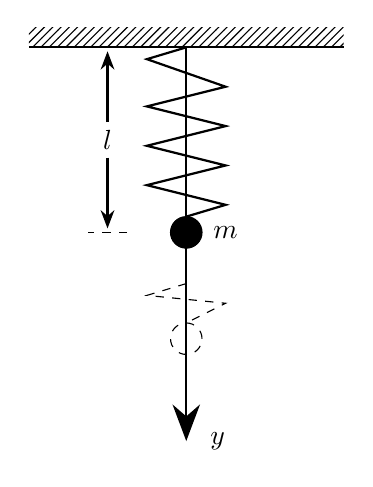
\begin{tikzpicture}
			\pattern[pattern=north east lines] (0,0) rectangle (4,.25);
			\draw[thick] (0,0) -- (4,0);
			\draw[thick,-{Stealth[scale=2]}] (2,0) -- (2,-5);
			\draw[thick] (2,0) -- (1.5,-.15) -- (2.5,-.5) -- (1.5,-.75)--(2.5,-1)--(1.5,-1.25)--(2.5, -1.5)--(1.5,-1.75)--(2.5, -2)--(2,-2.15);
			\draw[fill] (2,-2.35) circle [radius =0.2];

			\draw[dashed] (2,-3)--(1.5, -3.15)--(2.5,-3.25)--(2, -3.5);
			\draw[dashed] (2,-3.7) circle [radius =0.2];

			\draw[dashed] (1.25,-2.35) -- (0.75,-2.35);

			\node at (1,-1.175) {$l$};
			\draw[thick,-{Stealth[scale=1]}] (1,-1.4) -- (1,-2.3);
			\draw[thick,-{Stealth[scale=1]}] (1,-.95) -- (1,-.05);

			\node at (2.5,-2.35) {$m$};
			\node at (2.4,-5) {$y$};
		\end{tikzpicture}
		%
		\caption{Elastic spring of equilibrium length $l$ with an attached mass $m$.}
	\end{figure}

	Measuring the coordinate $y$ from the ceiling downwards, the mass is subject to a force
	equal to the sum of three contributions: the position-independent \textbf{gravity force} $f_g = mg$, the position dependent \textbf{elastic force} $f_{el} = −k(y − l)$ (Hook’s law of elasticity), and the \textbf{friction force} $f_a = - \gamma \dot{y}$ which is proportional to the velocity and is directed against the actual motion. Then (2) takes the form
	%
	\begin{equation}
			m\ddot{y} = mg - k(y-l)-\gamma \dot{y}\ .
	\end{equation}
	%
	Here $g$ is the gravity acceleration, $k$ is the spring constant depending on the spring’s material, and $\gamma$ is the friction coefficient. We will be able to analyze this equation and the resulting motion in due time, after we learn the methods allowing one to solve such equations.\par
	%
	\textbf{Example:}
	Another example in biology is the logistic equation, which is also called the Verhulst model. The logistic equation describes a model of population growth introduced by Pierre Verhulst (1845, 1847). In this model, the initial stage of population growth is approximately exponential when the population size $N$ is small; then the growth slows when population size increases, and stops when the population size reaches the maximum capacity of the environment $K$. The change of population size over time is governed by a first order non-linear differential equation.
	%
	\begin{equation}
			\frac{dN(t)}{dt} = rN(t)(1-\frac{N(t)}{K}).
	\end{equation}
	%
	Here, $r$ is the per capita growth rate of a population in the time interval $dt$. We can see that when $N(t) = K,\ \frac{dN(t)}{dt} = 0$, the population stops growing and its size does not change further. In biology, the maximum population size $K$ is called as the carrying capacity of a population under a certain environment. For some species, e.g. elephants in tropic forests, the carrying capacity $K$ can be very small such as hundreds, as elephants need a lot of food and large space and thus limited number of individuals can be afforded by a natural habitat. However, if we think of colon cancer population in our body, the carrying capacity $K$ can be as large as more than $10^11$ cells, as our body cell is very small, a detectable nail size tumour has more than $10^9$ cells. In this case, the initial growth of a tumour from a single cell can be approximately as exponential growth, where $N(t)/K \to 0$ when $t$ is small and $N(0) = 1$.

	\begin{figure}[!h]
		\centering
			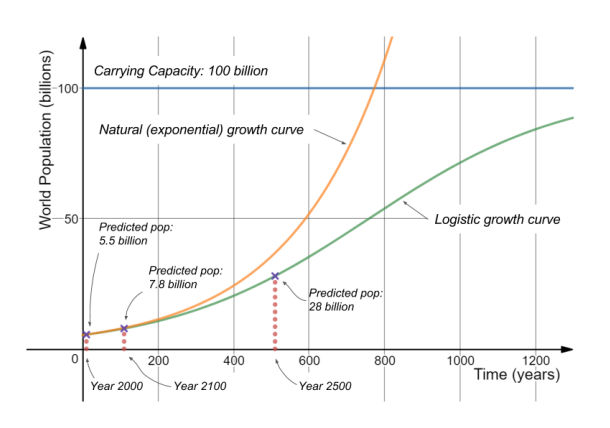
\includegraphics[width=0.75\textwidth]{steemiteducation.PNG}
			\caption{A illustrative figure of world population growth (from steemiteducation website).}
	\end{figure}

	%command for section, subsection and page on header
	\numberwithin{equation}{section}
	\pagestyle{fancy}
	\fancyhead[LE,RO]{\thepage}
	\fancyhead[RE]{\nouppercase \leftmark}
	\fancyhead[LO]{\nouppercase \rightmark}

	\section{Properties of first-order ODEs}
	\textbf{Explicit Solutions of Simple Types of First Order ODEs}\par 
	In this chapter we familiarize ourselves with a few simple \textbf{first-order differential equations}, always written in the \textbf{normal form} $y^\prime = f(x, y)$ or $\dot{y} = f(t, y)$, which allow for a complete analytical solution. The simplest case is one when the right-hand side is independent of $y$, that is
	$$
	y^\prime = f(x)
	$$
	Solutions to such an equation amount to finding the antiderivative for the right-hand side, that is, to a simple integration: $y = \int f(x) dx + C$, where $C$ is an arbitrary constant. We will see that general solutions of first order ODEs will always contain an arbitrary constant. The above type belongs in fact to a more general class of explicitly solvable first order ODEs as discussed in the next section.

	\subsection{Separable First Order ODEs}
	These are equations with the \textbf{right-hand side being a product of two factors}, one
	depending only on the variable $x$ and another one depending only on the unknown function $y$, that is
	%
	\begin{equation}
			\frac{dy}{dx} = f(x)g(y),
	\end{equation}
	%
	where both $f(x)$ and $g(y)$ are assumed to be continuous. The first observation is that if $y_1, \ldots , y_k$ are roots of the algebraic equation $g(y) = 0$, then the constant functions
	$$
	y(x) = y_1,\ y(x) = y_2,\ \ldots ,\ y(x) = y_k
	$$
	are solutions of the ODE (1.1).\\
	To find non-constant solutions scientists and engineers usually employ the following heuristic method (i.e mathematically ill-defined, but producing sensible results) of \textbf{separation of variables}, which allows one to solve (1.1) by the following steps: One starts with treating the derivative $\frac{dy}{dx}$ as if it was a ratio of two algebraic quantities $dy$ and $dx$. That way one formally \textit{separates variables} as $\frac{dy}{g(y)} = f(x) dx$ and by integrating both sides arrives at the
	relation
	%
	\begin{equation}
			\int \frac{dy}{g(y)} = \int f(x)dx + C,
	\end{equation}
	%
	where $C$ is an arbitrary constant. Denoting the result of integration on the left-hand side as $\frac{dy}{g(y)} \equiv H(y)$  (1.2) takes the form $H(y) = \int f(x)dx + C$. At the final step we may try to express $y(x)$ by formally defining the \textbf{inverse function} $H^{-1}(u)$ in such a way that $H(H^{-1}(u)) = u$, which is equivalent to
	$$
	H(y) = u \quad \Leftrightarrow \quad y = H^{-1}(u). 
	$$
	This allows one to write a one-parameter family of solutions to (1.1) as
	$$
	y = H^{-1}\left(\int f(x)dx + C \right).
	$$
	\textbf{Note:} There may exist more than one function inverse to a given function. For example, suppose $H(y) = y^2$. Solving $y^2 = u$ we find $y = \pm \sqrt{u}$ for any $u > 0$. Hence there exist two different inverse functions $H^{-1}(u > 0) = \sqrt{u}$ and $H^{-1}(u > 0) = -\sqrt{u}$. To find all solutions to an ODE by separation of variables we need to use all possible inverse functions $H^{-1}(u)$.\par
	\textbf{Example:}\\
	Find non-constant solutions of the ODEs
	$$
	\text{(\textbf{a})}\ y^\prime = xy^2, \qquad
	\text{(\textbf{b})}\ y^\prime = \frac{2xy}{1+y}, \qquad
	\text{(\textbf{c})}\ y^\prime = 3y^{3/2}
	$$
	\textbf{Solution:}\\

	\begin{enumerate}[(a)]
			\item Separating the variables we have
			$$
			H(y) = \int \frac{dy}{y} = \int xdx + C
			$$
			which gives $H(y) = -\frac{1}{y}$ on the left-hand side so that the equation $H(y) = -\frac{1}{y} = u$ is solved by $y = -1/u$. This defines the inverse function $H^{-1}(u)= -1/u$.  On the right-hand side the integration gives $\frac{1}{2}x^2 + C$.\\
			The general solution to the ODE is then given by applying the function to the right-hand side
			$$
			y = H^{-1}\left(\frac{x^2}{2}+C\right) = - \frac{1}{\frac{x^2}{2}+C}.
			$$
			for any value of the constant C.
			\item In this case
			$$
			H(y) = \int dy \frac{y+1}{2y}
			= \int x dx
			= \frac{1}{2}x^2 + C
			$$
			We further write on the left-hand side
			$$
			H(y) = \int dy \frac{y + 1}{2y}
			= \int dy\left[\frac{1}{2}+\frac{1}{2y}\right]
			= \frac{y}{2} + \frac{1}{2}\ln \left\lvert y\right\rvert
			$$
			However, in this case it is not possible to solve $\frac{y}{2} + \frac{1}{2}\ln \left\lvert y\right\rvert = u$ explicitly, so we neither can write an explicit formula for the inverse function $H^{-1}(u)$, nor find the general solution $y(x)$ explicitly. In such a case it is conventional to say that the general solution to the ODE is
			given in \textit{implicit} form by the relation $\frac{y}{2} + \frac{1}{2}\ln \left\lvert y\right\rvert = \frac{1}{2}x^2 + C$.
			\item To find the general solution valid for $y \ne 0$, we define $H(y) = \int \frac{dy}{3y^{2/3}} = y^{1/3}$,  so that solving $H(y) = y^{1/3} = u$ defines the inverse function $H^{-1} (u) = u^3$. As $f(x) = 1$ we have on the right-hand side $\int f(x)dx = x + C$. Finally, the general solution is given by applying the inverse $H^{−1}$ to the right-hand side: $y = H^{−1}(x + C) = (x + C)^3$.\par
			It is easy to check by direct substitution that the heuristic ”separation of variables” method indeed works perfectly, but a mathematician must be concerned with finding a justification of the correct results obtained by an ill-defined method. A mathematically legitimate way of solving (1.1) goes as follows. Let the equation $g(y) = 0$ have distinct real roots $y = y_1 < y_2 < y_3 \ldots $. so that $y(x) = y_1,\ y(x) = y_2$, etc. are solutions to (1.1) (which are called in this case special solutions). Consider now any open interval $(A, B)$ which contains none of the
			roots $y_1, y_2,\ldots $. Then $g(y) \ne 0$ for any $y \in (A, B)$ (that is $g(y)$ retains its sign inside the interval). Then inside the interval we can rewrite (1.1) as
			%
			\begin{equation}
					\frac{1}{g(y)}y^\prime = f(x)
			\end{equation}
			%
			Define the function $H(y)$ via the indefinite integral:
			$$
			H(y) = \int \frac{1}{g(y)}dy.
			$$
			and consider a function of variable $x$ defined as $H(y(x))$. Then using the chain rule of differentiation we have
			%
			\begin{equation}
					\frac{d}{dy}H(y(x))
					= \frac{dH}{dy}\frac{dy}{dx}
					= \frac{1}{g(y)}y^\prime = f(x)
			\end{equation}
			%
			so that we conclude that $H(y(x))$ is an antiderivative of $f(x)$, hence
			$$
			H(y(x)) = \int f(x)dx + C.
			$$
			Since $g(y)$ retains its sign in $(A, B)$ the derivative $\frac{dH}{dy} = \frac{1}{g(y)}$ is of the same sign in the interval. Therefore the function $H(y)$ is either strictly increasing, or strictly decreasing in $(A, B)$, hence it has a unique functional inverse $H^{−1}$ inside that interval. The general solution $y(x)$ of (1.1) is therefore given by
			%
			\begin{equation}
					y(x) = H^{-1}\left(\int f(x)dx + C\right)
			\end{equation}
			%
			and indeed coincides with one predicted by the heuristic method.
	\end{enumerate}

	\subsection{First order ODEs which can be reduced to be separable}
	\begin{enumerate}
			\item Consider equations of the type
			
			\begin{equation}
					y^\prime = f(ax + by + c), \qquad \text{where $a,\ b,\ c$ are real constants}
			\end{equation}
			Introducing a new function $z(x) = ax + by + c$ we see that this equation can be rewritten as $y^\prime = f(z)$. Then (1.6) becomes equivalent to
			%
			\begin{equation}
					z^\prime = a + by^\prime = a + bf(z),
			\end{equation}
			%
			which is a particular type of separable equation (1.1).\par
			\textbf{Example:}\\
			Solve the equation
			$$
			y^\prime = (4y − x − 6)^2
			$$
			\textbf{Solution:}
			We introduce $z = 4y − x − 6$ so that the equation can be written as $y^\prime = z^2$ Then $z^\prime = 4y^\prime − 1 = 4z^2 − 1$ which is a separable ODE. Separating variables we get
			$$
			\int \frac{dz}{4z^2-1} = \int dx + C
			$$
			and performing the integration in the left-hand side as:
			$$
			H(z) = \frac{1}{2}\int \left(\frac{1}{2z-1}-\frac{1}{2z+1}dz\right)
			$$
			we see that
			$$
			H(z)
			= \frac{1}{4}(\ln \left\lvert 2z − 1 \right\rvert - \ln \left\lvert 2z + 1 \right\rvert)
			= \frac{1}{4} \ln \left\lvert \frac{2z − 1}{2z + 1}\right\rvert 
			$$
			The inverse function $H^{−1}(u)$ is obtained by solving $H(z) = u$, that is
			$$
			\frac{1}{4} \ln \left\lvert \frac{2z − 1}{2z + 1}\right\rvert
			\quad
			\Leftrightarrow 
			\quad
			\left\lvert \frac{2z − 1}{2z + 1}\right\rvert
			= e^{4u}
			$$
			Solving for $z$ (exercise for yourself!) gives explicitly two possible solutions
			$$
			z(u) = \frac{1}{2}\frac{1+e^{4u}}{1-e^{4u}}
			\quad
			\text{or}
			\quad
			z(u) = \frac{1}{2}\frac{1-e^{4u}}{1+e^{4u}}.
			$$
			Denoting the functions on the right-hand side as $z = H^{−1}(u)$ we see that the solution $z(x)$ is given in either case by
			$$
			z(x)
			= H^{-1}(x+C)
			= \frac{1}{2}\frac{1\pm e^{4(x+c)}}{1\mp e^{4(x+c)}}
			$$
			It is convenient to write $\pm e^{4C} = A$, where the constant $A$ may have an arbitrary sign. Finally, using the definition of $z$ we see that $y$ is expressed in terms of the above $z$ via
			$$
			y
			= \frac{1}{4}(z(x) + x + 6)
			= \frac{1}{4}\left(x + 6 + \frac{1}{2}\frac{1 + Ae^{4x}}{1 - Ae^{4x}}\right)
			$$
			which gives the general solution to the original ODE.
	\end{enumerate}
\end{document}